% =====================================================================
% MATH-454 Parallel and High Performance Computing -- Final project
% Slides: Lattice Boltzmann 2D flow past a cylinder (MPI + CUDA)
% Clean 16:9 beamer deck, EPFL logo. 4 slides as required by the handout.
% Build: pdflatex slides.tex   (run twice for the page counter)
% =====================================================================
\documentclass[aspectratio=169,10pt]{beamer}

% --- Clean, sober look ---
\usetheme{default}
\usefonttheme{professionalfonts}
\usepackage[T1]{fontenc}
\usepackage{lmodern}
\usepackage{helvet}            % sans-serif body for a clean modern look
\renewcommand{\familydefault}{\sfdefault}
\usepackage{graphicx}
\usepackage{tikz}
\setbeamertemplate{navigation symbols}{}  % remove navigation clutter

% --- EPFL-style accent colour ---
\definecolor{epflred}{RGB}{200,16,46}
\definecolor{darkgray}{RGB}{60,60,60}
\setbeamercolor{frametitle}{fg=epflred}
\setbeamercolor{structure}{fg=epflred}
\setbeamercolor{normal text}{fg=darkgray}
\setbeamerfont{frametitle}{series=\bfseries}
\setbeamertemplate{itemize item}{\color{epflred}\textbullet}
\setbeamertemplate{itemize subitem}{\color{epflred}\textendash}

% --- Frame title: bold title + thin red rule underneath ---
\setbeamertemplate{frametitle}{%
  \vspace{0.4em}%
  \begin{minipage}{0.80\paperwidth}%
    \usebeamerfont{frametitle}\usebeamercolor[fg]{frametitle}\insertframetitle%
  \end{minipage}\\[0.15em]%
  {\color{epflred}\rule{0.92\paperwidth}{1.2pt}}%
}

% --- EPFL logo top-right on every slide ---
\setbeamertemplate{background}{%
  \begin{tikzpicture}[remember picture,overlay]
    \node[anchor=north east, inner sep=10pt] at (current page.north east)
      {
\includegraphics[height=6mm]{figures/epfl_logo.pdf}};
  \end{tikzpicture}%
}

% --- Footer: name / course / slide number ---
\setbeamertemplate{footline}{%
  \hbox{}\vspace{2pt}%
  \hspace{0.4cm}\footnotesize\color{darkgray}%
  Simon Pierre \,\textbar\, MATH-454 \,\textbar\, LBM with MPI \& CUDA%
  \hfill\insertframenumber/\inserttotalframenumber\hspace{0.4cm}%
  \vspace{4pt}%
}

% Helper for a small caption line under the points
\newcommand{\takeaway}[1]{\vspace{0.3em}{\color{epflred}\footnotesize\textbf{Takeaway:} #1}}

\begin{document}

% =====================================================================
% SLIDE 1 -- MPI strong scaling vs Amdahl
% =====================================================================
\begin{frame}{MPI strong scaling vs Amdahl}
  \begin{columns}[T]
    \begin{column}{0.46\textwidth}
      \footnotesize
      \textbf{Setup:} fixed grid, ranks $P=1\ldots128$, three sizes;
      speedup $S(P)=\mathrm{MLUPS}(P)/\mathrm{MLUPS}(1)$.
      \medskip
      \begin{itemize}\setlength\itemsep{0.45em}
        \item Profiling: serial fraction $s<1\%$ (only parsing + the
          single-point probe) $\Rightarrow$ Amdahl predicts \emph{near-linear}
          speedup.
        \item We follow it at low $P$, then bend away at high $P$.
        \item The gap is \textbf{not} an Amdahl serial fraction (constant)
          but \textbf{communication} + \textbf{memory bandwidth}, which grow
          in relative weight with $P$.
        \item Surface-to-volume: compute $\propto n_y/P$ rows, halo
          $\propto 2$ rows $\Rightarrow$ thin slabs communicate too much.
      \end{itemize}
      \takeaway{deviation from ideal is a hardware effect, not a serial part.}
    \end{column}
    \begin{column}{0.54\textwidth}
      \centering
      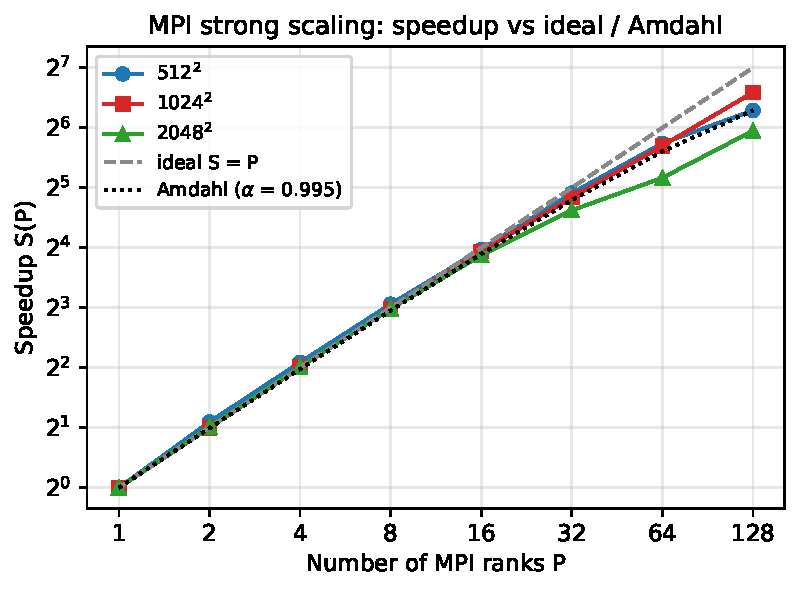
\includegraphics[height=0.66\textheight]{../plotting/figures/mpi_strong_speedup.pdf}
    \end{column}
  \end{columns}
\end{frame}

% =====================================================================
% SLIDE 2 -- MPI weak scaling vs Gustafson
% =====================================================================
\begin{frame}{MPI weak scaling vs Gustafson}
  \begin{columns}[T]
    \begin{column}{0.46\textwidth}
      \footnotesize
      \textbf{Setup:} constant work per rank (128 rows/rank, $n_y=128P$).
      Gustafson with tiny $s$ predicts a \emph{flat} efficiency.
      \medskip
      \begin{itemize}\setlength\itemsep{0.4em}
        \item Measured efficiency falls $100\%\to39\%$. Three distinct causes:
        \item \textbf{(1)} $P{=}1\!\to\!2$: a \textbf{cache} effect, not comm.
          The small per-rank domain keeps $P{=}1$ in the shared L3 (28.6 vs
          $\sim$21 MLUPS for strong $P{=}1$); at $P{=}2$ two cores share it
          and lose the boost.
        \item \textbf{(2)} $P{=}8\ldots64$ (one node): shared
          \textbf{memory-bandwidth saturation} -- the dominant limiter, since
          LBM is memory-bound; \emph{not} the communication.
        \item \textbf{(3)} $P{=}128$: crossing onto a \textbf{second node}
          (inter-node network) past 72 cores.
      \end{itemize}
      \takeaway{absolute throughput still grows $28.6\to1434$ MLUPS.}
    \end{column}
    \begin{column}{0.54\textwidth}
      \centering
      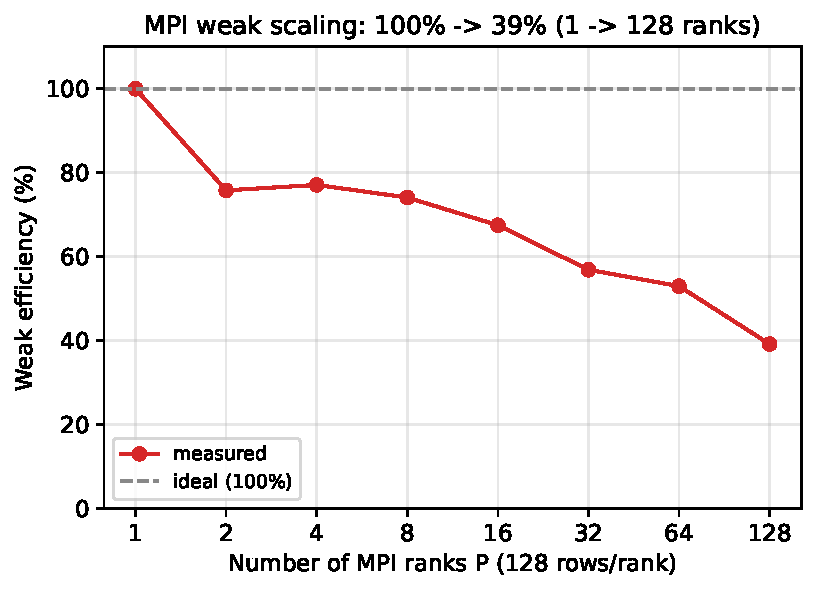
\includegraphics[height=0.66\textheight]{../plotting/figures/mpi_weak.pdf}
    \end{column}
  \end{columns}
\end{frame}

% =====================================================================
% SLIDE 3 -- CUDA: memory layout and roofline
% =====================================================================
\begin{frame}{CUDA on a V100: memory layout is everything}
  \begin{columns}[T]
    \begin{column}{0.46\textwidth}
      \footnotesize
      \textbf{Design:} one thread per cell, one kernel per phase, double
      buffering for streaming, \emph{no} communication on a single GPU.
      \textbf{2051 MLUPS} $\approx 101\times$ the serial baseline; $St=0.16$.
      \medskip
      \begin{itemize}\setlength\itemsep{0.4em}
        \item LBM is \textbf{memory-bound}: roofline $\approx 3100$ MLUPS
          ($288$ B/LUP, $\sim900$ GB/s). We reach $\sim66\%$ of it.
        \item \textbf{SoA vs AoS $=3.6\times$} (the headline): SoA lets a warp
          \emph{coalesce} its loads; AoS scatters them across cache lines.
        \item Block-size sweep: broad plateau $128$--$512$ (occupancy, not the
          ceiling). Size sweep: up to $\sim81\%$ of the roofline at $4096^2$.
      \end{itemize}
      \takeaway{for a memory-bound code the access pattern dominates.}
    \end{column}
    \begin{column}{0.54\textwidth}
      \centering
      \vspace{0.5em}
      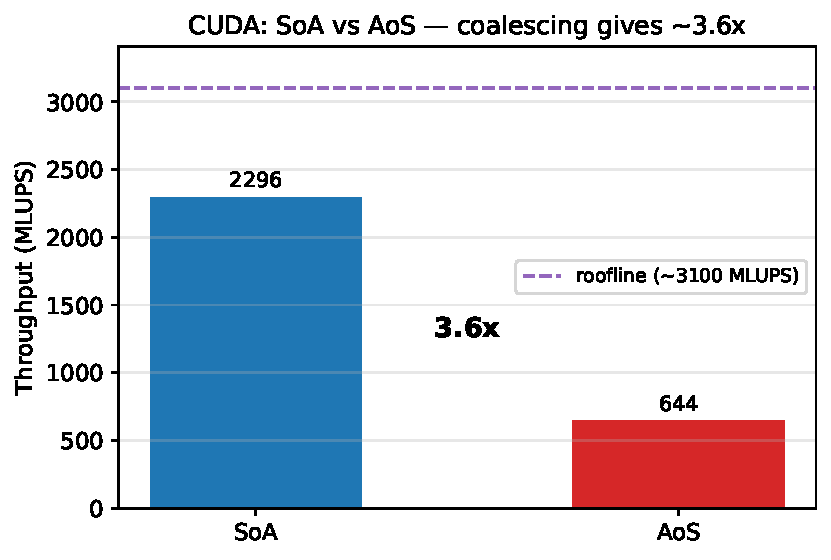
\includegraphics[height=0.66\textheight]{../plotting/figures/cuda_layout.pdf}
    \end{column}
  \end{columns}
\end{frame}

% =====================================================================
% SLIDE 4 -- Free choice: the strong-scaling crossover
% =====================================================================
\begin{frame}{Free choice: the strong-scaling crossover}
  \begin{columns}[T]
    \begin{column}{0.46\textwidth}
      \footnotesize
      The same strong-scaling data, read as \textbf{efficiency} $E(P)$, tells
      a richer story than ``bigger scales better''.
      \medskip
      \begin{itemize}\setlength\itemsep{0.4em}
        \item \textbf{Super-linear} at low $P$ ($E>100\%$): the subdomain
          starts to fit in \textbf{cache}, so each core speeds up -- not an error.
        \item At high $P$, two \emph{opposite} limiters:
        \item $512^2$ becomes \textbf{communication-bound} (4 rows/rank,
          exchange 2) $\to 61\%$.
        \item $2048^2$ becomes \textbf{bandwidth-bound} (drops $32\!\to\!64$
          \emph{within} one node) $\to 56\%$.
        \item $1024^2$ is the \textbf{sweet spot} $\to 75\%$.
      \end{itemize}
      \takeaway{trade-off: comm.\ likes large grids, cache/bandwidth likes
      small; ``bigger always scales better'' is only half true ($2048^2$ is
      bandwidth-limited).}
    \end{column}
    \begin{column}{0.54\textwidth}
      \centering
      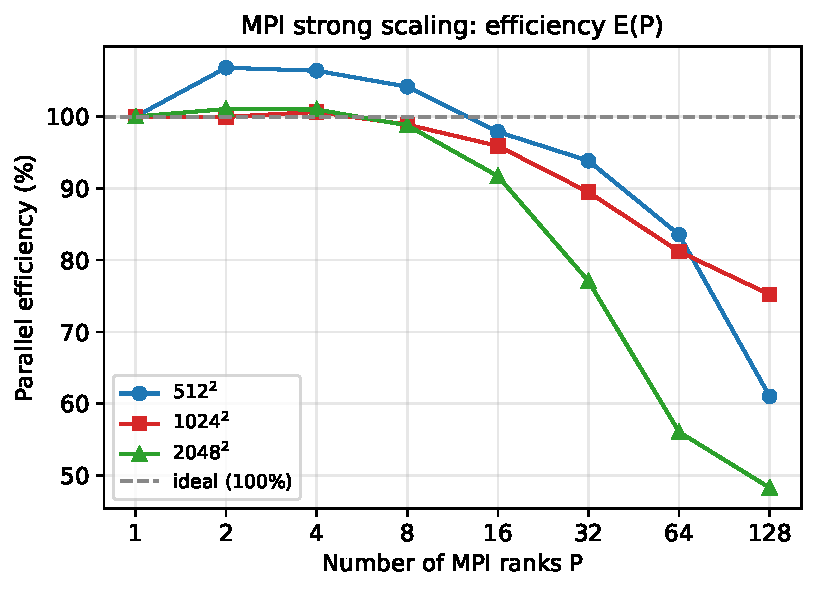
\includegraphics[height=0.66\textheight]{../plotting/figures/mpi_strong_efficiency.pdf}
    \end{column}
  \end{columns}
\end{frame}

\end{document}
